\documentclass[12pt]{ctexart}
\usepackage[utf8]{inputenc}
\usepackage[T1]{fontenc}
\usepackage{graphicx}
\usepackage{xcolor}
\usepackage{float}
\usepackage{hyperref}
%%novalidate

\usepackage{tikz}
\usepackage{calc}
\usepackage{booktabs}


% colors
\definecolor{color1}{HTML}{000060}
%\definecolor{color1}{HTML}{8C260F}
\definecolor{color2}{HTML}{333333}


% fonts
\usepackage{fontspec}
\defaultfontfeatures{Mapping=tex-text}
\setmainfont
[BoldFont=Lato-Bold.ttf,
ItalicFont=Lato-Italic.ttf,
BoldItalicFont=Lato-BoldItalic.ttf]
{Lato-Regular.ttf}
\newfontfamily\headingfont[ItalicFont=Lato-BlackItalic.ttf]{Lato-Black.ttf}
%%%

\usepackage{geometry}
\geometry{a4paper,
hmargin=20mm,vmargin=20mm,
head=0ex,foot=3ex}

\linespread{1.3}

\usepackage[hang]{caption}
\DeclareCaptionFormat{upper}{#1#2\uppercase{#3}\par}
\captionsetup{labelfont={bf,color=color2},textfont={normalsize,color=color2},format = upper,figurename=图,tablename=表}

%%% fancy sections
\usepackage{titlesec}
%\titleformat{\chapter}{\headingfont\LARGE\bfseries\scshape\color{color1}}{\thechapter}{1em}{}[\titlerule]
\titleformat{\section}{\color{color1}\headingfont\Large\bfseries\uppercase}{\thesection}{1em}{}[\titlerule]
\titleformat{\subsection}{\color{color1}\headingfont\large\bfseries\uppercase}{\thesubsection}{1em}{}
\titleformat{\subsubsection}{\color{color1}\headingfont\bfseries\uppercase}{\thesubsubsection}{1em}{}
%%%

% head and foot
\usepackage{fancyhdr}
\pagestyle{fancy}
\lhead{}
\chead{}
\makeatletter
\rhead{\color{color2}\@date}
\makeatother
\newlength{\myheight}
\lfoot{
\settoheight{\myheight}{\thepage}
\raisebox{-2ex-0.5\myheight}{
\includegraphics[height=4ex]{logo}}
}
\cfoot{\color{color2}肺龄焕新商业计划书}
\rfoot{\color{color2}\thepage}
\renewcommand\headrulewidth{0pt}
\renewcommand\footrulewidth{0pt}

% custom titlepage
\makeatletter
\newcommand*\DefVar[1]{\@namedef{#1}##1{\global\@namedef{get#1}{##1}}}
\DefVar{summary}
\renewcommand{\maketitle}{
\begin{center}

\begin{tikzpicture}
    \node[draw=none,%color1,line width=0.4pt,
      fill=color1,
      inner sep = 10pt,
      text width=\textwidth-20pt,
      text centered
    ] {\color{white}\headingfont\bfseries\huge\@title};
\end{tikzpicture}
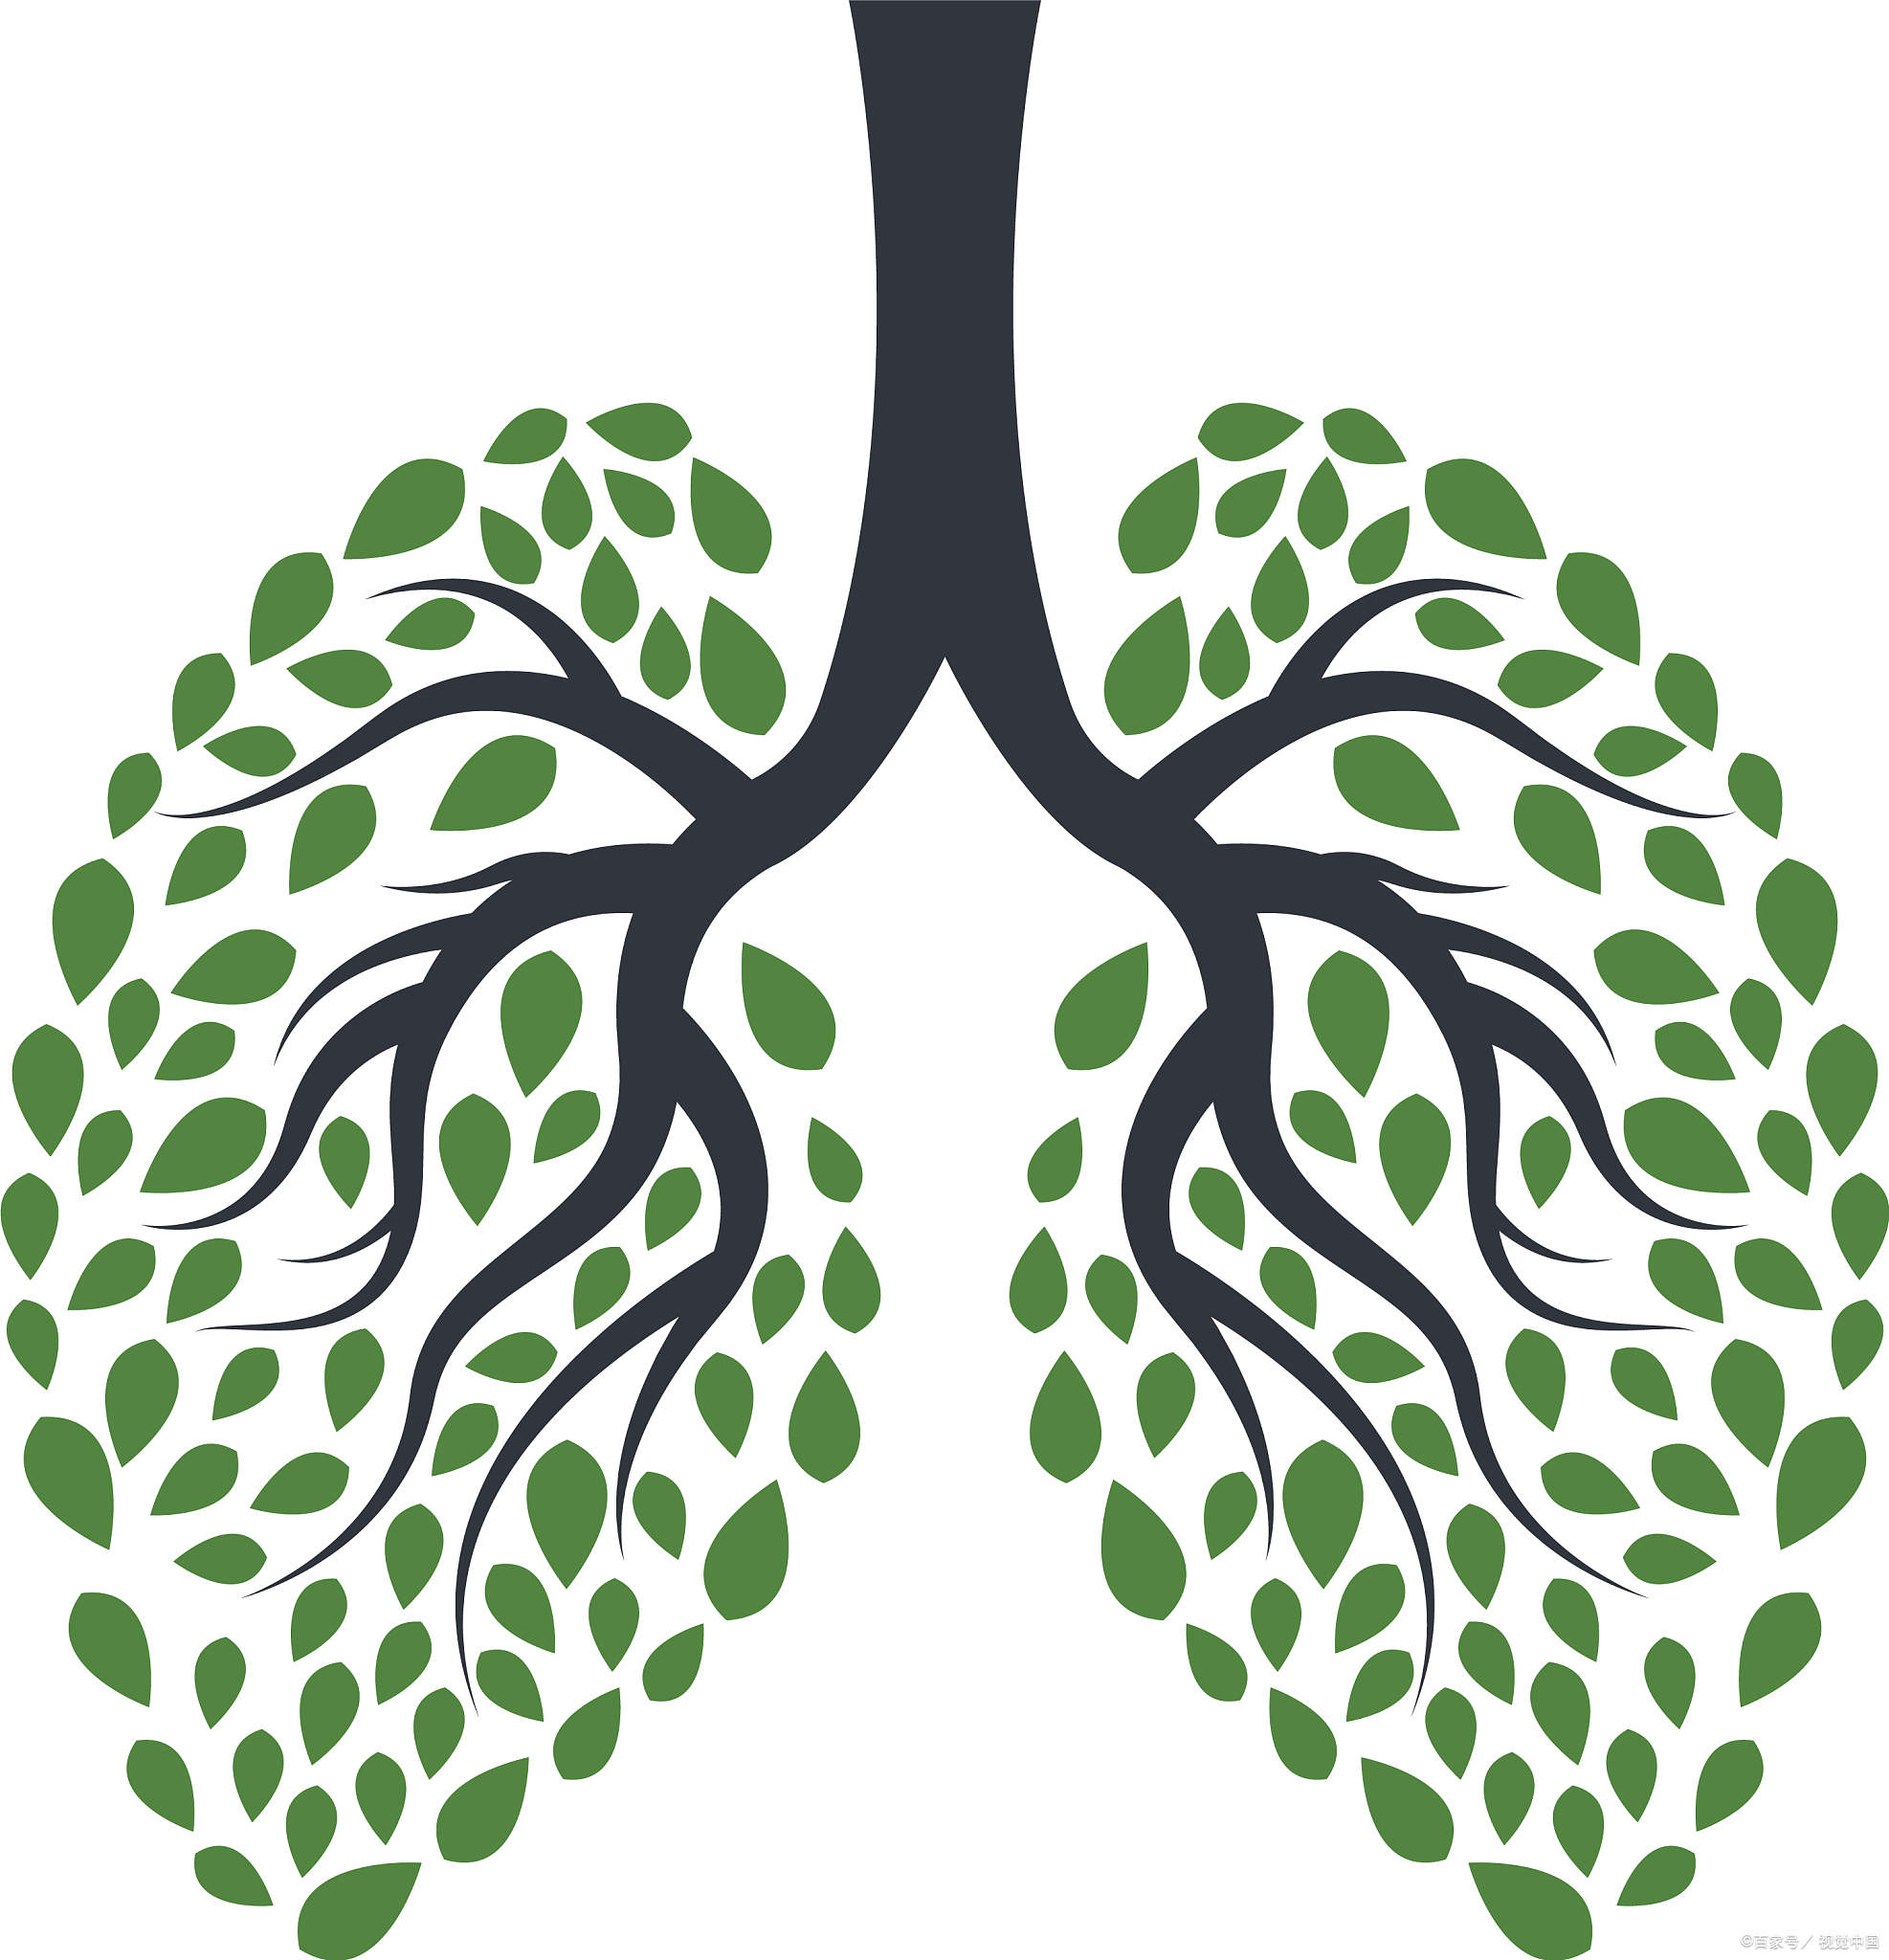
\includegraphics[width=\textwidth]{opening}\par
\headingfont\bfseries\Large\@author\par
\bigskip\medskip
{\color{color2}\normalfont\normalsize%\textbf{口号:}\\
\getsummary}
\end{center}
\clearpage
}
\makeatother
%%%

%%% fancy boxes
\usepackage{tcolorbox}
\usepackage{wrapfig}
\def\fullboxbegin{
\bigskip
\begin{tcolorbox}[colback=color1,colframe=color1,coltext=white,arc=0mm,boxrule=0pt]
}
\def\fullboxend{\end{tcolorbox}\medskip}
%
\def\leftboxbegin{
\begin{wrapfigure}{l}{0.5\textwidth}
\begin{tcolorbox}[colback=color1,colframe=color1,coltext=white,arc=0mm,boxrule=0pt]
}
\def\leftboxend{
\end{tcolorbox}
\end{wrapfigure}
}
%
\def\rightboxbegin{
\begin{wrapfigure}{r}{0.5\textwidth}
\begin{tcolorbox}[colback=color1,colframe=color1,coltext=white,arc=0mm,boxrule=0pt]
}
\def\rightboxend{
\end{tcolorbox}
\end{wrapfigure}
}
%
\newcounter{frames}
\def\frameboxbegin#1{
\bigskip
\refstepcounter{frames}
\begin{tcolorbox}[colback=white,colframe=color1,arc=0mm,title={\MakeUppercase{\textbf{\arabic{frames}}: #1}}]
}
\def\frameboxend{
\end{tcolorbox}
}
%%%
\usepackage[backend=biber,style=gb7714-2015, autocite=footnote, citestyle=verbose]{biblatex}
\addbibresource{./ref.bib}
\hypersetup{
colorlinks=true,
linkcolor=blue,
filecolor=magenta,
urlcolor=cyan,
pdftitle={商业计划书},
pdfpagemode=FullScreen,
}
%%%%%%%%%%%%%%%
% Title Page
\title{\textbf{肺龄焕新}商业计划书}
\author{创业实践第八组}
\date{\today}
\summary{
焕活肺动力,呼吸更年轻!
}
%%%%%%%%%%%%%%%

\begin{document}
\maketitle

\tableofcontents
\clearpage

\section{概览}
\subsection{摘要}
\begin{itemize}
    \item \textbf{核心问题提炼:}

    现有市场缺乏能有效对抗自由基、深度修复肺部氧化损伤的预防及治疗肺结节的产品。

    \item \textbf{我们的初步构想:}

    “肺龄焕新”是一款基于接骨木莓等高效抗氧化成分,
    并运用靶向技术减少肝首过效应的肺部健康产品,旨在提供卓越的肺部抗氧化和保护效果。

    \item \textbf{市场机遇:}

    呼吸系统疾病高发且持续增长,政策支持健康中国战略及慢性呼吸系统疾病防治,国民健康意识和医疗支出提升。

    \item \textbf{待验证的关键假设:}
    目标用户群体(如吸烟人群、中老年)对提升肺部抗氧化能力有强烈需求并愿意为此付费。

\end{itemize}
\section{问题与机遇}
\subsection{目标用户画像及痛点}

\subsubsection{中老年养生群体}
\paragraph{基本特征}
年龄在 45-70 岁,注重身体健康,有较强的养生意识,退休后有充足时间关注自身健康,部分人有慢性病管理经验。
\paragraph{健康需求}
因年龄增长,肺部功能逐渐衰退,易受雾霾、二手烟等环境因素影响,常出现咳嗽、气短等症状,希望通过保健品预防肺部疾病,改善呼吸功能。
\paragraph{消费习惯}
信赖传统药店、医院推荐的产品,倾向选择口碑好、品牌历史悠久的保健品,对价格敏感度较低,但重视产品安全性和有效性,愿意为优质产品支付较高费用。
\subsubsection{职场高压吸烟人群}
\paragraph{基本特征}
主要为 25-45 岁的男性,工作压力大,应酬频繁,有长期吸烟习惯,吸烟史 3-15 年不等,部分人意识到吸烟对肺部健康的危害,但戒烟困难。
\paragraph{健康需求}
因长期吸烟,肺部积累大量有害物质,担心引发肺癌、慢性阻塞性肺病等严重疾病,希望通过保健品减轻吸烟对肺部的损伤,缓解咳嗽、咽干等不适症状。
\paragraph{消费习惯}
多通过电商平台、社交媒体了解产品信息,偏好便捷的线上购物方式,对产品包装设计、服用便捷性有一定要求,注重产品功效宣传的科学性和专业性,愿意尝试新品牌和新产品。
\subsubsection{户外运动爱好者}
\paragraph{基本特征}
年龄在 18-40 岁,热爱跑步、骑行、登山等户外运动,经常在户外环境中暴露于灰尘、花粉、汽车尾气等污染物中,对自身健康和体能状态关注度高。
\paragraph{健康需求}
为减少户外运动时吸入的污染物对肺部造成的损害,预防呼吸道感染,保持良好的肺部功能以支持运动表现,需要具有防护和修复功能的保健品。
\paragraph{消费习惯}
活跃于运动社群、健身 APP 等平台,容易受运动达人、网红推荐影响,倾向购买天然成分、无副作用的产品,注重产品便携性,愿意为具有运动健康理念的品牌支付溢价。
\subsubsection{环境污染敏感型人群}
\paragraph{基本特征}
生活在工业发达城市或雾霾严重地区,年龄跨度较大(20-60 岁),对空气质量变化敏感,部分人患有过敏性鼻炎、哮喘等呼吸道疾病,易因环境污染诱发或加重病情。
\paragraph{健康需求}
急需通过保健品增强肺部对污染物的抵抗力,减轻环境污染对肺部的氧化损伤,缓解呼吸不畅、过敏等症状,降低呼吸道疾病发作频率。
\paragraph{消费习惯}
通过环保资讯平台、健康科普公众号获取产品信息,关注产品成分中抗氧化、抗炎的功效描述,对产品安全性要求极高,愿意为针对环境污染设计的专业肺部保健品买单。


\subsection{行业痛点}
\fullboxbegin
呼吸系统疾病是一种常见病、多发病。
其疾病种类复杂,主要病变在气管、支气管、肺部及胸腔,主要症状为咳嗽、胸痛、痰多、呼吸受影响,严重者出现呼吸困难、缺氧,甚至呼吸衰竭而死亡。
根据国家统计局数据显示,呼吸系统疾病已成为中国第三大疾病死因,仅次于心脑血管疾病和恶性肿瘤。
\fullboxend
首先,由于工业化进程加速、环境污染加剧、近几年疫情带来的巨大冲击以及吸烟等不良生活习惯的影响,我国慢性呼吸系统和肺部疾病发病率在不断上升。目前慢性呼吸系统疾病的死亡人次占比超过八成,全球2021年呼吸系统和肺部疾病患病病例数约为187亿人次,预计2025年将增至203亿人次,慢性呼吸系统及肺部疾病病例数呈现持续上升趋势。

其次,目前市场上多数肺部保健品主要采用常见的中药材、维生素以及部分天然提取物等成分。
例如一些产品以百合、银耳等传统养肺食材为主,虽有一定润肺功效,但在对抗自由基、深度修复肺部氧化损伤方面作用有限。
维生素类产品,如维生素 C,抗氧化能力较弱,难以应对复杂环境下肺部遭受的高强度自由基攻击。即便部分产品添加槲皮素这一具有抗氧化、抗炎作用的黄酮类化合物,但其在保健品中的应用仍存在局限性。一方面,槲皮素水溶性差、生物利用度低,口服后难以在体内达到有效浓度,导致其抗氧化、抗炎等护肺功效大打折扣;另一方面,单一的槲皮素难以应对肺部面临的多因素损伤,缺乏协同作用机制,无法从多维度对肺部进行全面保护。

因此,市场上仍然缺乏一种能够有效实现肺部抗氧化的护肺产品。

\subsection{市场机会与初步验证}
\subsubsection{政策层面}
为贯彻党中央关于实施健康中国战略的决策部署,落实《国务院关于实施健康中国行动的意见》《健康中国行动(2019—2030年)》要求,深入开展慢性呼吸系统疾病防治工作,提高我国居民呼吸健康水平,我国制定《健康中国行动——慢性呼吸系统疾病防治行动实施方案(2024—2030年)》。《方案》要求完善慢性呼吸系统疾病防治体系建设,动员全社会参与慢性呼吸系统疾病及其危险因素全程管理,倡导健康生活方式,普及健康知识,中西医并重,加强慢性呼吸系统疾病的早筛、早诊和早治,加强政策引导和资源配置,有效遏制慢性呼吸系统疾病增长带来的危害,增强人民群众健康获得感,为共建共享健康中国奠定重要基础。到2030年,慢性呼吸系统疾病防治体系进一步完善,危险因素综合防控取得阶段性进展,慢性呼吸系统疾病基层筛查能力及规范化管理水平显著提升,70岁及以下人群慢性呼吸系统疾病死亡率下降到8.1/10万及以下。

同时,国际社会对呼吸疾病的重视与日俱增,我国在其中承担着特殊而重要的角色。2019年第13届全球防治慢性呼吸疾病联盟(GARD)会议在中国召开,同期发布《国际肺部健康促进行动北京宣言》(以下简称“北京宣言”),呼吁社会各方共同协作,积极开展呼吸疾病防治的工作,从全新的视角提出了对慢性呼吸疾病的防治工作要求。

国内国际相互联动,为我国肺部健康行业发展提供了政策背书。
\subsubsection{经济层面}
\paragraph{国民收入和医疗保健支出增长为呼吸系统和肺部疾病药物行业注入发展活力。}

近年来,我国居民可支配收入呈现逐年稳定增长态势,进而带动医疗大健康产业发展,医疗保健消费支出占比随着收入增长而明显提升。根据国家统计局数据,2022年我国人均可支配收入达3.7万元,人均医疗保健消费支出达2120元,人均医疗保健消费支出占人均消费总支出的8.6\%,相较于2012年提高了1.6\%。因此,随着人们对医疗健康的重视程度越来越高,对医疗健康的支出意愿也不断增强,为呼吸系统和肺部疾病药物行业进一步发展奠定了坚实的需求基础。

\paragraph{呼吸系统和肺部疾病药物行业市场规模不断扩大}

如图\ref{fig:market_growth},2021年全球呼吸系统和肺部疾病药物市场规模为1294亿美元,2015-2021年复合年增长率为 2.8\%,预计2030年市场规模将达到1837亿美元;2021年呼吸系统和肺部疾病药物全球市场规模为 2718亿元,2015-2021年复合增长率为6.9\%,预计2030 年市场规模将达到4531亿元,2021-2030年年复合增长率为5.8\%。

\begin{figure}[H]
    \centering
    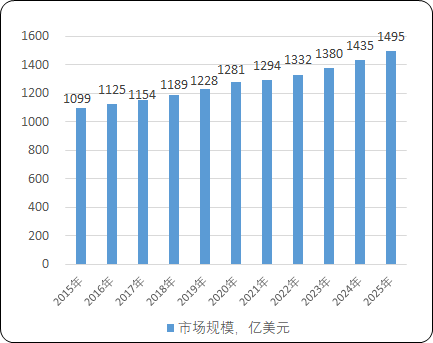
\includegraphics[width=0.8\textwidth]{./fig/市场.png}
    \caption{呼吸系统和肺部疾病药物市场规模增长}
    \label{fig:market_growth}
\end{figure}
\subsubsection{社会层面}
\paragraph{呼吸系统和肺部疾病患者数量持续增加,带来庞大的药物及保健品市场需求。}

随着环境变化、人口老龄化趋势、生活方式转变等因素的影响,国民的肺部健康面临着严峻的挑战,我国慢性肺部疾病患病人群十分庞大,患病人数逐年增加。人们对肺部健康需求愈发强烈。
根据图\ref{fig:patient_growth}显示\autocite{data},2021年全球呼吸系统和肺部疾病患病病例数约为187亿人次,预计2030年将增至209亿人次,2021-2030年复合年增长率将保持1.2\%;中国呼吸系统和肺部疾病患病病例数约为28亿人次,预计2030年将增至30亿人次,2021-2030年复合年增长率保持0.8\%。此外,呼吸系统疾病具有典型的年龄特征,我国人口老龄化趋势将会进一步扩大患病人群。
\begin{figure}[H]
    \centering
    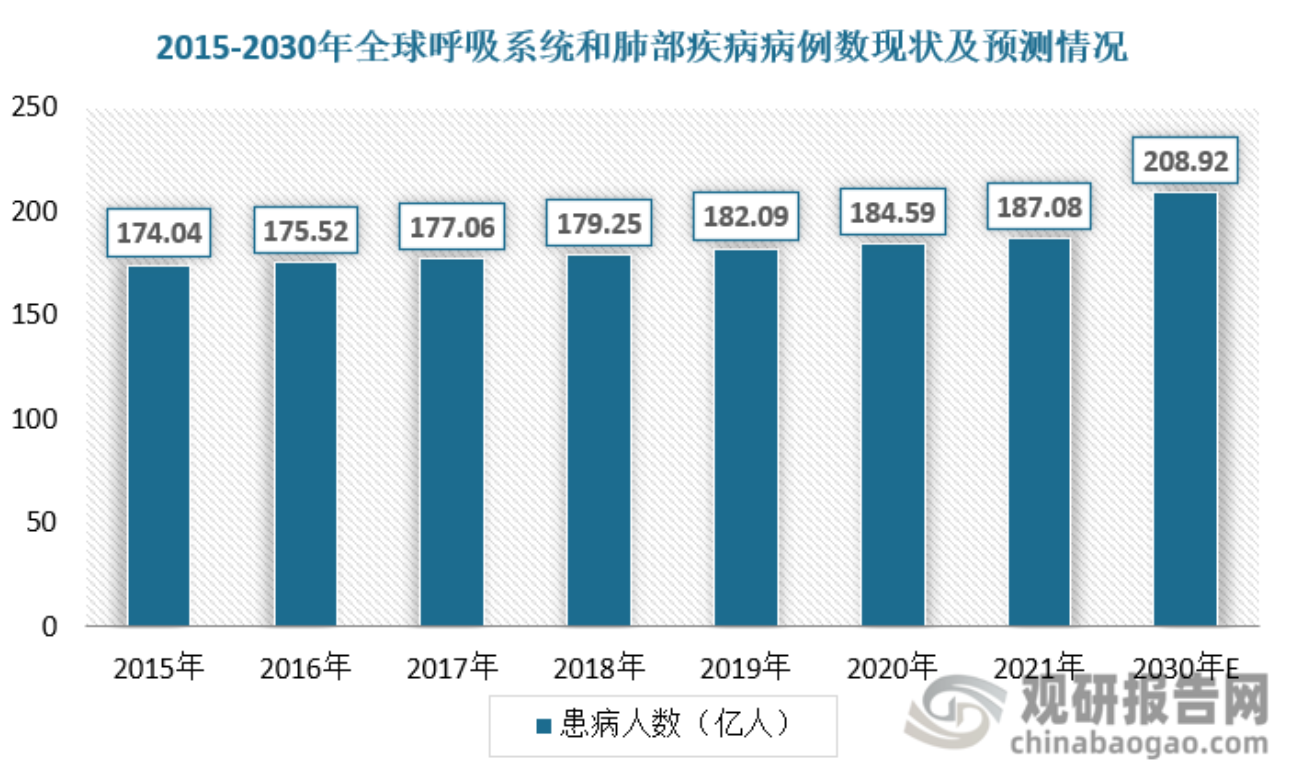
\includegraphics[width=0.8\textwidth]{./fig/病例数.png}
    \caption{呼吸系统和肺部疾病患者数量增长}
    \label{fig:patient_growth}
\end{figure}
\subsubsection{技术层面}
TODO
\section{解决方案与价值主张的迭代}
\subsection{原料采用}
接骨木莓(Elderberry)是接骨木属(学名:Sambucus)植物的果实,隶属于五福花科(Adoxaceae)\autocite{wiki_sambucus_2024} 。该属约有20余种,广泛分布于全球温带和亚热带地区,其中欧洲接骨木(Sambucus nigra,又称西洋接骨木或黑果接骨木)和美国接骨木(Sambucus canadensis)是较为常见且研究较多的品种\autocite{ucanr_elderplant_2021}。这些植物通常为灌木或小乔木,春夏季节会绽放出乳白色或淡黄色的花簇,随后在夏秋季结出深紫色或蓝黑色的浆果 。值得注意的是,接骨木属的植物学分类依据基因序列分析的APG分类法,已从原先的忍冬科(Caprifoliaceae)调整至五福花科,这体现了现代植物分类学的进展。不同品种在果实风味和生长习性上可能存在差异,例如美国接骨木的果实有时被认为更甜,且更耐热 。  

接骨木莓在世界各地拥有悠久的传统应用历史。早在古希腊时期,希波克拉底等就已记载其药用价值。
在欧洲民间医学中,接骨木莓常被用于缓解感冒、流感等上呼吸道感染症状,并作为增强免疫力的天然草药。
其花朵和浆果也被广泛用于制作果酱、糖浆、酒类及茶饮。

在中国传统医学中,特定种类的接骨木(如Sambucus williamsii Hance)的茎、枝等部位亦被入药,认为具有祛风湿、活血通络、
治疗跌打损伤及骨折等功效 。传统中医药对植物不同部位的运用,暗示了其对植物整体药用价值的广泛认知,
这与西方草药学主要关注浆果和花朵有所不同。  

现代科学研究揭示,接骨木莓富含多种生物活性化合物,其中花青素(Anthocyanins)和黄酮类化合物(Flavonoids)尤为引人注目。
花青素是赋予接骨木莓深邃紫黑色泽的主要色素,其含量据报道远高于蓝莓、黑醋栗等其他常见浆果,
约占总多酚含量的80\%\autocite{daiken_elderberry_nodate}。
主要的黄酮类化合物则包括槲皮素(Quercetin)和芸香苷(Rutin)等。
这些丰富的植物化学物质是接骨木莓诸多健康益处的物质基础。

得益于这些活性成分,接骨木莓表现出显著的抗氧化、抗炎、抗病毒(尤其针对流感病毒)以及免疫调节等生理功能\autocite{abed_elderberry_2023}。
多项研究表明,接骨木莓提取物能够增强机体对病毒的防御能力,
例如通过抑制病毒复制或阻止病毒进入宿主细胞,并可能通过刺激细胞因子产生来调节免疫反应。
其强大的抗氧化能力有助于中和体内自由基,减轻氧化应激损伤,而抗炎作用则有助于缓解炎症反应。
这些特性使其在辅助改善呼吸道健康、增强免疫力方面展现出应用潜力,并因此受到持续的科学关注。
世界卫生组织(WHO)和欧洲药品管理局(EMA)已将其列为具有呼吸道缓解和增强特性的治疗性辅助对症治疗选择。

综上所述,接骨木莓作为一种历史悠久的食药两用植物资源,凭借其独特的生物活性成分,
在传统医学和现代健康科学领域均占有重要地位。对其化学成分、药理作用及作用机制的深入研究,将有助于更全面地发掘其应用价值。

\subsection{技术革新}
\fullboxbegin
简单来说,肝脏首过效应(也叫首过代谢)指的是我们口服一些药物后,药物在被吸收到血液并到达全身发挥作用之前,会先经过我们的肝脏(有时也包括肠壁) 。在肝脏这个“第一关”,一部分药物会被肝脏里的酶“处理”掉(代谢掉),导致最终能真正进入血液循环发挥药效的药物量减少了 。

这就好比你寄一个包裹,包裹在到达最终目的地之前,先要经过一个中转站(肝脏),中转站的工作人员(肝脏里的酶)可能会打开包裹检查,并拿走一部分东西(药物被代谢)。所以,最后到达目的地的东西(进入血液的有效药物)就比你最初寄出的要少。

这个效应会直接影响药物的“生物利用度”,也就是我们吃了多少药,有多少能真正起作用 。如果一个药物的首过效应很强,意味着很多药物在肝脏就被“消耗”了,那么口服这种药时,可能就需要更大的剂量才能达到治疗效果,或者医生会建议通过其他不经过肝脏首过效应的给药途径,比如舌下含服或注射等 。

影响首过效应的因素有很多,比如药物本身的性质、个人的肝功能状况、肝脏内酶的活性(这和遗传有一定关系)以及同时服用的其他药物等 。
\fullboxend
而本产品可以减少肝首过效应,使得药物可以直达病灶,疗效较市场同类产品更好。
\section{商业模式探索}
\subsection{精益画布}
梳理出商业模式的关键要素,形成精益画布如图\ref{fig:lean_canvas},帮助团队更好地理解商业模式的各个方面。
\begin{figure}[H]
    \centering
    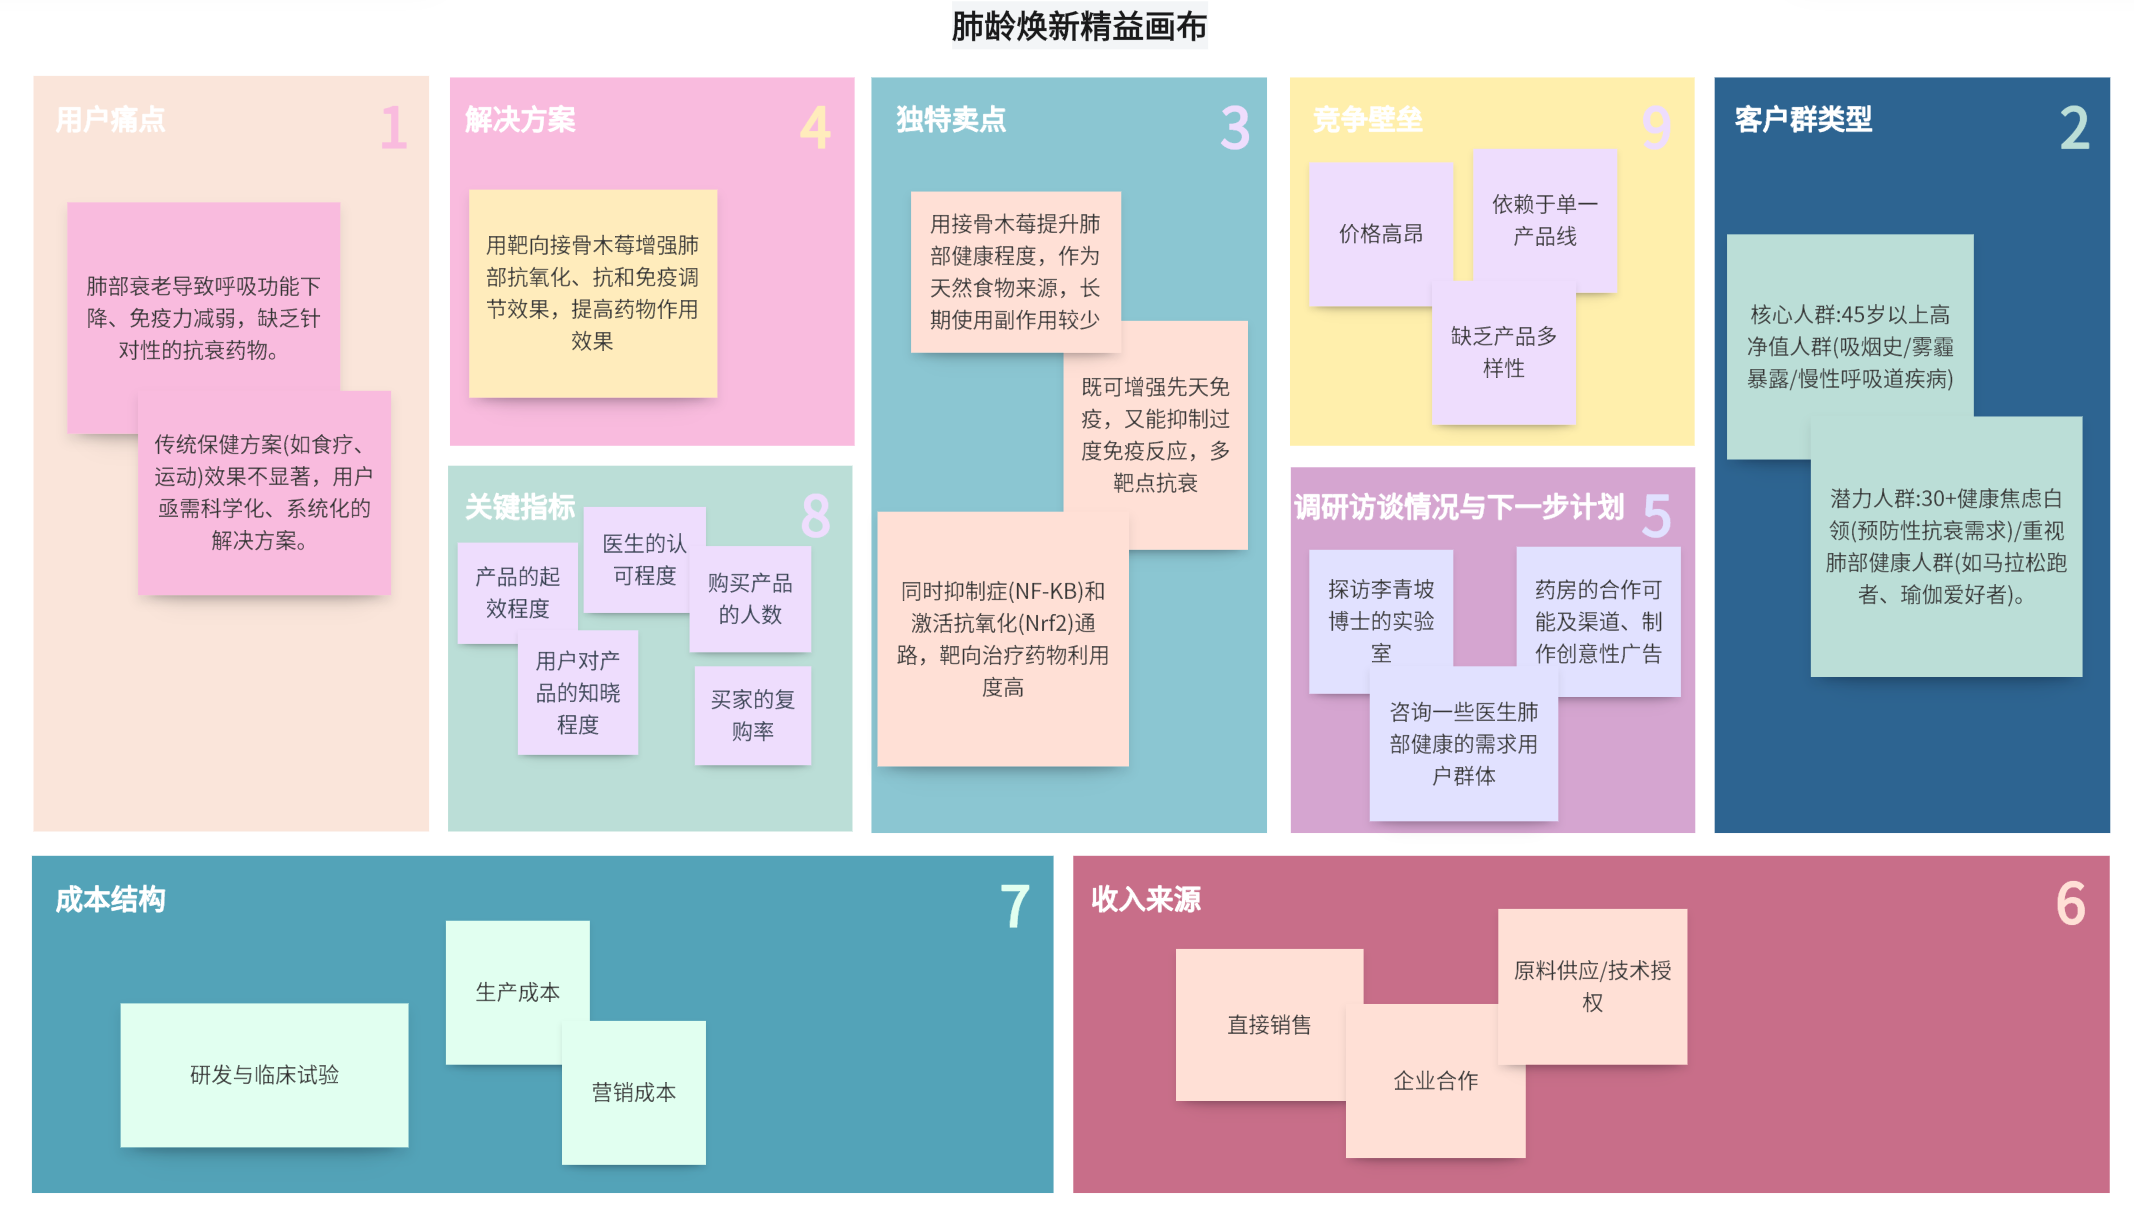
\includegraphics[width=0.9\textwidth]{./reference/精益画布.png}
    \caption{精益画布}
    \label{fig:lean_canvas}
\end{figure}
\subsection{拟定商业模式}
\subsubsection{CBEC营销}
充分利用平台提供的营销工具,结合KOL/KOC(关键意见领袖/关键意见消费者)推广,进行精准广告投放,并参与平台促销活动以吸引流量和转化。

CBEC无疑是多数外国保健品牌,特别是那些拥有创新成分或特定健康诉求(尚未被“蓝帽子”体系覆盖)的品牌的首选初始路径。天猫国际和京东国际作为两大头部平台,其选择可能取决于目标消费群体、成本预算和服务模式的偏好。然而,成功运营CBEC店铺不仅仅是简单上架产品,更需要积极的市场推广、对平台规则的深入理解,以及可能需要专业TP的协助。同时,接骨木莓花色苷的NFI审评进展 需持续关注,若其获批使得一般贸易更为便捷,可能会影响对CBEC模式的长期依赖。中国消费者对外国保健品的高需求 和CBEC平台提供的直接市场通路共同构成了这一模式的可行性基础,但平台运营成本 和激烈的市场竞争也要求企业制定清晰的投资回报策略。

\subsubsection{聚焦数字化的直达消费者(DTC)模式}
核心渠道与策略:
\begin{itemize}
    \item \textbf{微信生态系统:}
        \begin{itemize}
            \item \textbf{微信小程序:}

            是中国DTC模式的关键工具。它允许品牌在微信这一拥有超过13亿用户的平台内,提供个性化健康咨询、产品推荐、在线购买、内容分发和社群构建等一体化服务 。成功案例包括LemonBox(主打个性化维生素定制),以及Swisse、Blackmores等国际品牌也通过小程序进行用户互动和销售。
            \item \textbf{微信公众号:}

            作为内容营销和客户服务的基地,可以发布科普文章、品牌故事,并引导用户关注和使用小程序 。
        \end{itemize}
    \item \textbf{个性化补充剂与订阅服务:}

    这是全球保健品市场的一大趋势,并在中国市场由LemonBox等品牌成功实践。
    企业可以通过在线健康评估(收集用户的饮食习惯、生活方式、健康目标等信息),
    为用户推荐个性化的接骨木莓补充剂方案。订阅模式则能提供便利性并带来持续性收入。
    COVID-19疫情进一步催化了个性化免疫支持产品的需求。
    \item \textbf{品牌自建电商网站:}
    虽然可以作为微信生态的补充,但在中国市场,独立电商网站的流量获取成本高昂,挑战巨大,通常不作为主要的DTC销售渠道。
\end{itemize}

以微信为核心的DTC模式,为品牌提供了一个绝佳的平台,能够以合规的方式向消费者深入浅出地阐释接骨木莓对肺部抗氧化支持的益处,从而培养消费者的信任和忠诚度。个性化服务可以成为强大的独特销售主张(USP)。LemonBox通过微信小程序提供个性化维生素定制的成功案例 ,以及Swisse和Blackmores等品牌在微信生态的有效运营 ,都证明了此模式在中国市场的可行性。然而,这也要求企业在内容创作、社群运营、小程序开发与维护方面进行持续投入。小程序流量的获取将高度依赖于有效的社交媒体营销(如KOL/KOC合作、微信广告等)。中国的“私域流量”运营理念 与DTC模式高度契合,通过在微信内构建忠实的品牌社群,可以实现持续的用户互动,并相较于在大型公共电商平台不断竞争而言,能有效降低长期获客成本。

\subsubsection{未来趋势与长期增长战略}

未来市场趋势研判:
\begin{itemize}
    \item 个性化营养:消费者对根据个体需求定制的健康方案的需求日益增长 。接骨木莓补充剂未来可作为个性化健康组合包的一部分。
    \item 传统中医(TCM)理念的融合:将天然草本植物成分与现代科学相结合的产品,更容易获得中国消费者的青睐。可探索接骨木莓在TCM理论中是否有相符的健康叙事。
    \item 细分人群的精准定位:针对老年人、都市白领、健身爱好者等特定人群的需求,进行产品配方和市场营销的定制化。
    \item 先进配方与递送系统:在生物利用度、靶向效果等方面的技术创新将持续受到关注。
\end{itemize}
\section{执行与产品迭代}
\subsection{调研}
计划先从校医院医生及校医学院学生开始进行实地访谈,了解他们对肺部健康的看法和需求,及对该技术可行性的分析。
结合专利申请过程及相关文献的调研,完成对接骨木莓治疗药的包装初步设计。
\subsection{迭代}
设计MVP:
“肺龄焕新基础抗氧胶囊”——核心成分(如高活性接骨木莓提取物+优化槲皮素),基础生产工艺,小批量生产。

核心验证假设: 社区群体在试用MVP 4周后,能感知到初步的体感改善(如咳嗽减轻、呼吸较顺畅等)。

实验设计: 招募30-50名目标用户,进行双盲或开放标签试用,通过问卷、访谈收集反馈。

成功指标: 用户反馈及购买意愿。
\section{关键风险与应对策略}

\end{document}
